\section{Teilversuch 1: Aufbau des Foldscopes}
	\begin{tabularx}{\textwidth}{l p{1mm} X}
		\toprule
		\tou{Versuchsziel} && Aufbau des Foldscopes \\
		\tou{Messmethode} && Augenmaß \\
		\bottomrule
	\end{tabularx}
	\subsection{Linsengleichung für eine biconvexe Linse}
		Für eine Linse mit brechenden Kugelflächen gilt die allgemeine Linsenschleiferformel \citep{kling_96_nodate}:
		\begin{equation}
			\frac{1}{f} = \left(\frac{n_L}{n_M} - 1\right)\left(\frac{1}{R_1} - \frac{1}{R_2} + \frac{\left(\frac{n_L}{n_M} - 1\right)d}{\frac{n_L}{n_M}R_1R_2}\right)
		\end{equation}
		mit \hspace{1cm}
		\begin{tabular}{ll}
			$f$   & Effektive Brennweite der Linse vom Zentrum \\
			$n_L$ & Brechungsindex vom der Linse \\
			$n_M$ & Brechungsindex von das umgebende Medium \\
			$R_1$ & Krümmungsradius der Eintrittsfläche (mit Vorzeichen) \\
			$R_2$ & Krümmungsradius der Austrittsfläche (mit Vorzeichen) \\
			$d$   & Dicke der Linse
		\end{tabular}

		Für eine biconvexe Linse ist $R_1 > 0$ und $R_2 < 0$. Da wir die Linse nur im Luft verwenden, ist $n_M \approx 1$, wie wir im Versuch MZI bestätigt haben. Schreibe $\frac{n_L}{n_M}$ als $n$, dann erhalten wir:
		\begin{equation}
			\frac{1}{f} = \left(n - 1\right)\left(\frac{1}{R_1} - \frac{1}{R_2} + \frac{\left(n - 1\right)d}{nR_1R_2}\right)
		\end{equation}
		Wir verwenden in diesem Versuch eine Kugellinse, somit ist $\abs{R_1} = \abs{R_2} = R$ und $d = 2R$. Somit ergibt sich:
		\begin{align}
			\frac{1}{f} 
			&= \left(n - 1\right)\left(\frac{1}{R} + \frac{1}{R} - \frac{\left(n - 1\right)(2R)}{nR^2}\right) \notag \\ 
			&= \left(n - 1\right)\left(\frac{2}{R} - \frac{\left(2n - 2\right)R}{nR^2}\right) \notag \\
			&= \left(n - 1\right)\left(\frac{\cancel{2n} - \left(\cancel{2n} - 2\right)\cancel{R}}{nR\cancel{^2}}\right) \notag \\
			&= \frac{2(n-1)}{nR}
		\end{align}
		Daraus ergibt sich die effektive Brennweite:
		\begin{align}
			f = \frac{nR}{2(n-1)} = \frac{nD}{4(n-1)} \label{eqn:focallength}
		\end{align}
		wobei $D$ der Durchmesser ist. 

		Es gilt außerdem unter der paraxiellen Näherung die Gleichung:
		\begin{align}
			\frac{1}{f} = \frac{1}{g} + \frac{1}{b}
		\end{align}
		mit \hspace{1cm}
		\begin{tabular}{ll}
			$f$   & Effektive Brennweite der Linse vom Zentrum \\
			$g$   & Gegenstandsweite \\
			$b$   & Bildweite
		\end{tabular}

	\subsection{Fotoprotokoll des Aufbaus}
		Anhand der beiliegenden Anleitung (Siehe Anhang \ref{appdx:anleitung}) wurde das Foldscope aufgebaut. Die hier dokumentierte Schritten entsprechen die Schritten in der Anleitung.
		\vfill
		\begin{center}
			\begin{tabular}{*{3}{l}}
				% \toprule
				\multicolumn{1}{l|}{Schritt 1} & Schritt 2 & $\rightarrow$\\
				\midrule
				\multicolumn{1}{l|}{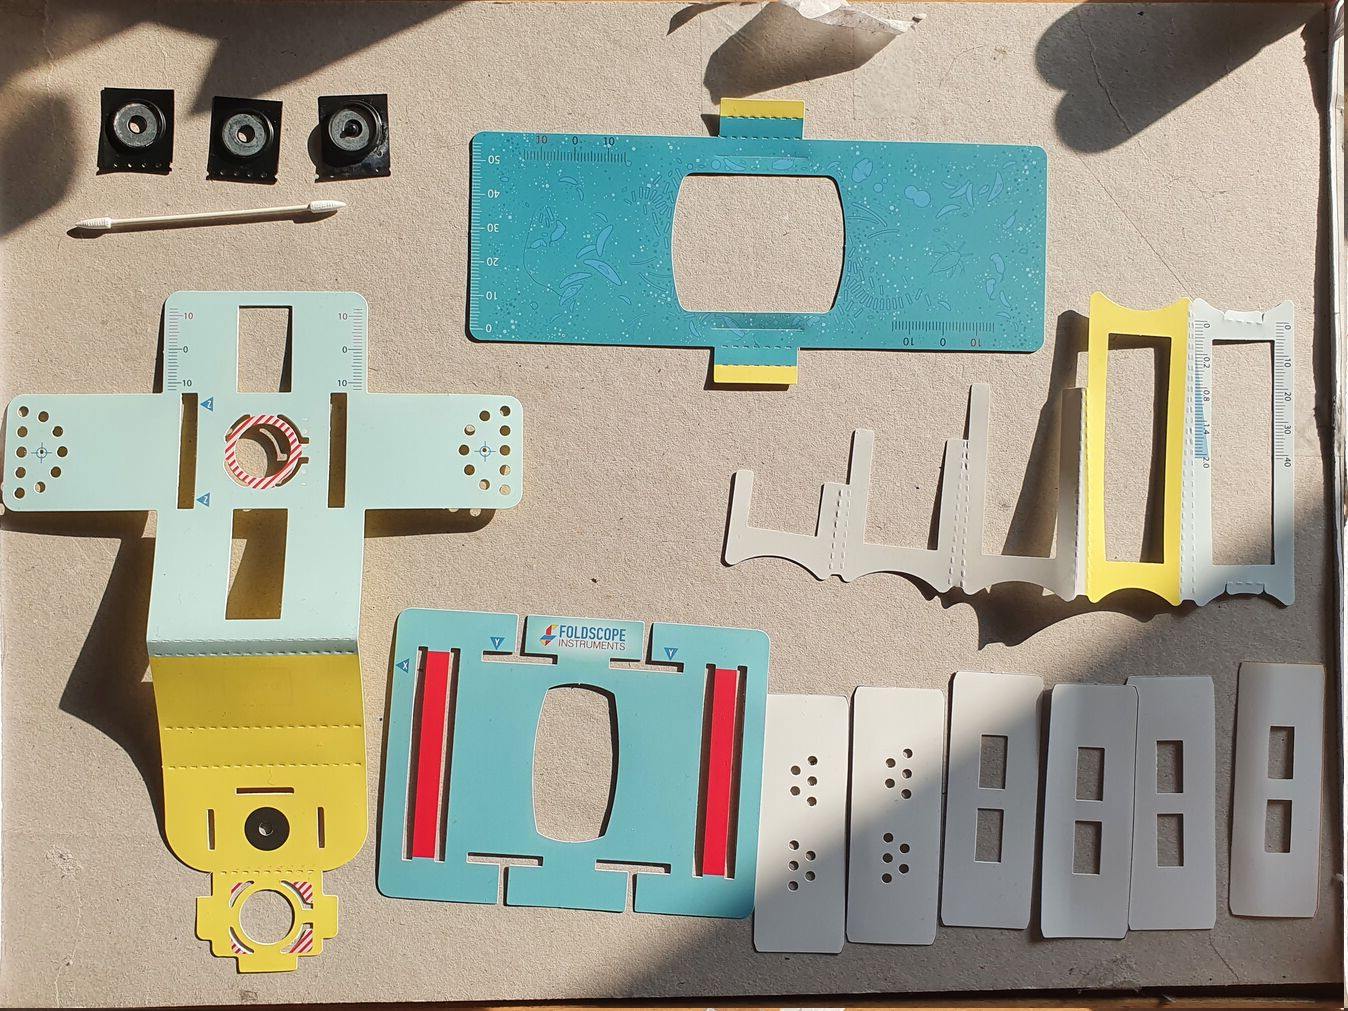
\includegraphics[width=0.3\textwidth]{images/aufbau/1_1.jpg}} & 
				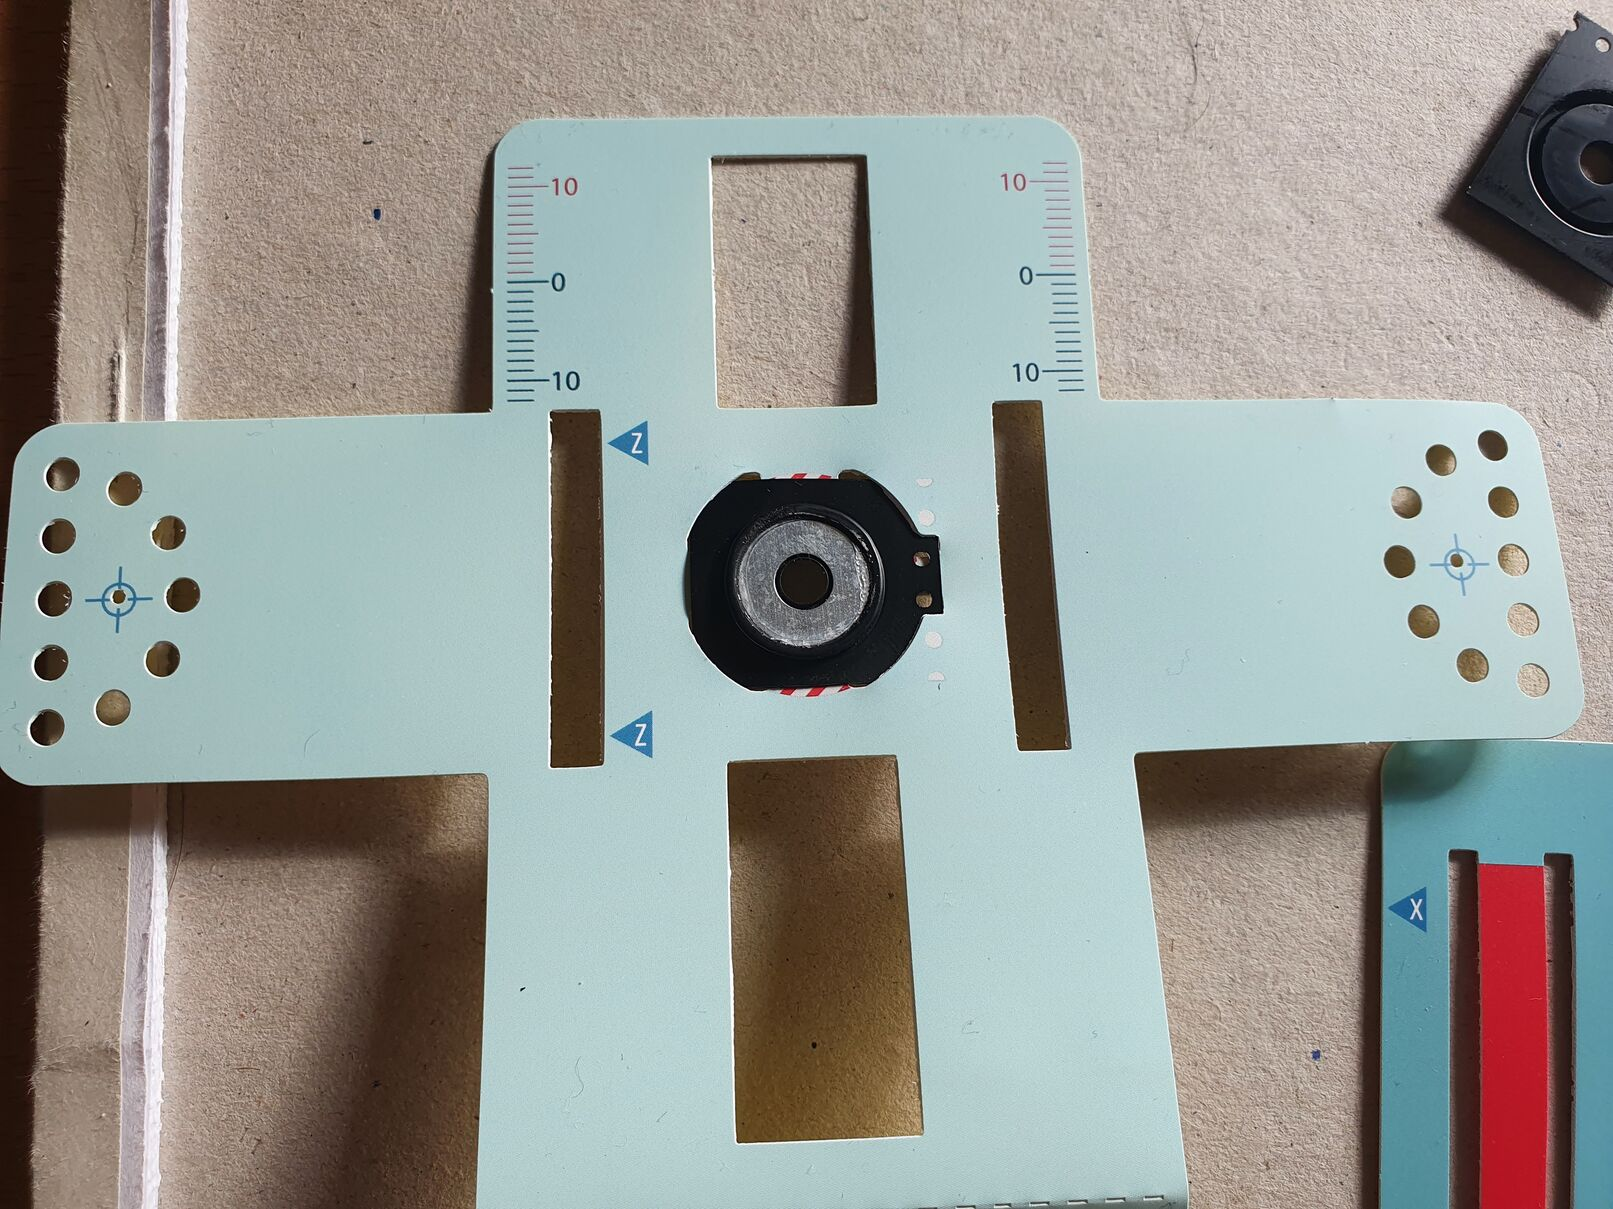
\includegraphics[width=0.3\textwidth]{images/aufbau/2_1.jpg} & 
				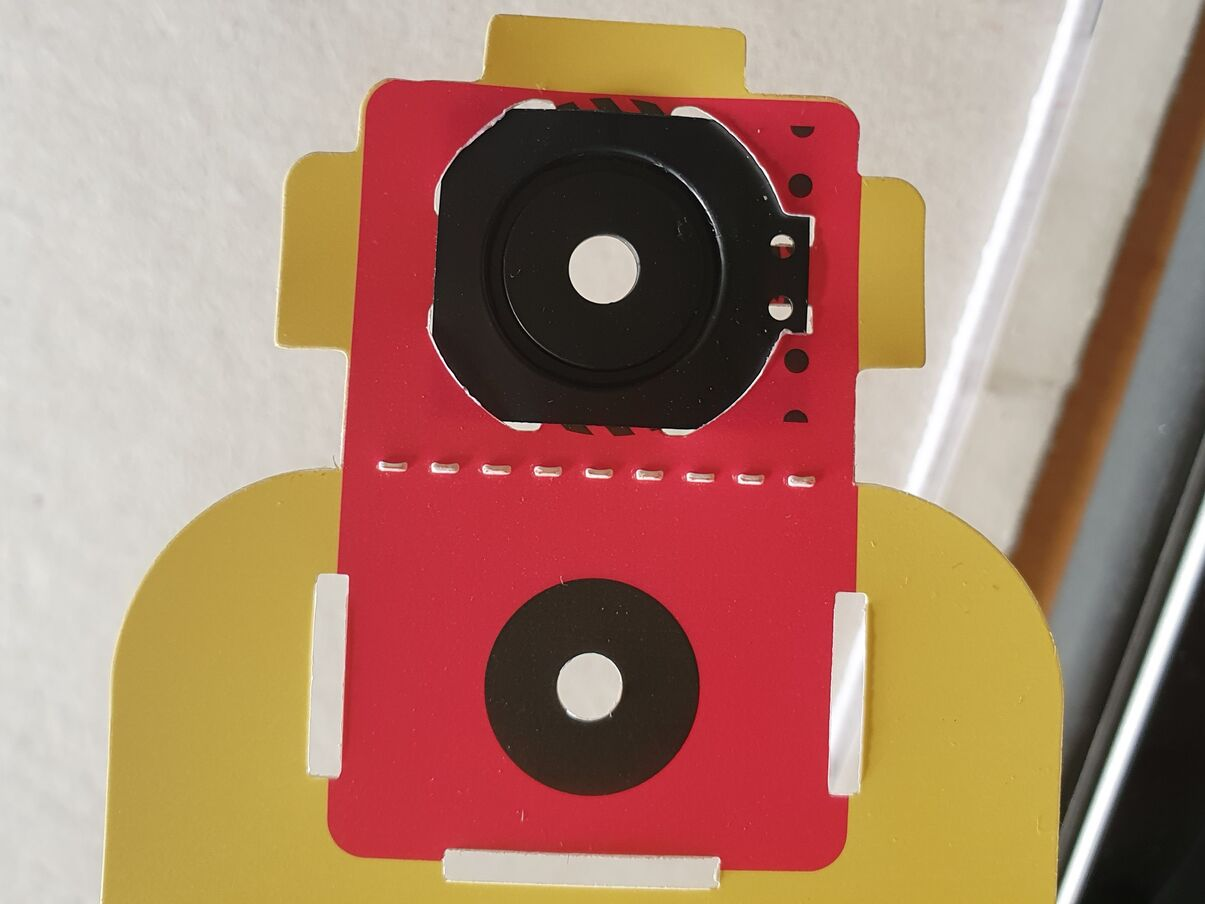
\includegraphics[width=0.3\textwidth]{images/aufbau/2_2.jpg} \\
				% \bottomrule 
				\\[-0.5em]
				% \toprule
				$\rightarrow$ & \multicolumn{1}{l|}{$\rightarrow$} & Schritt 3 \\
				\midrule
				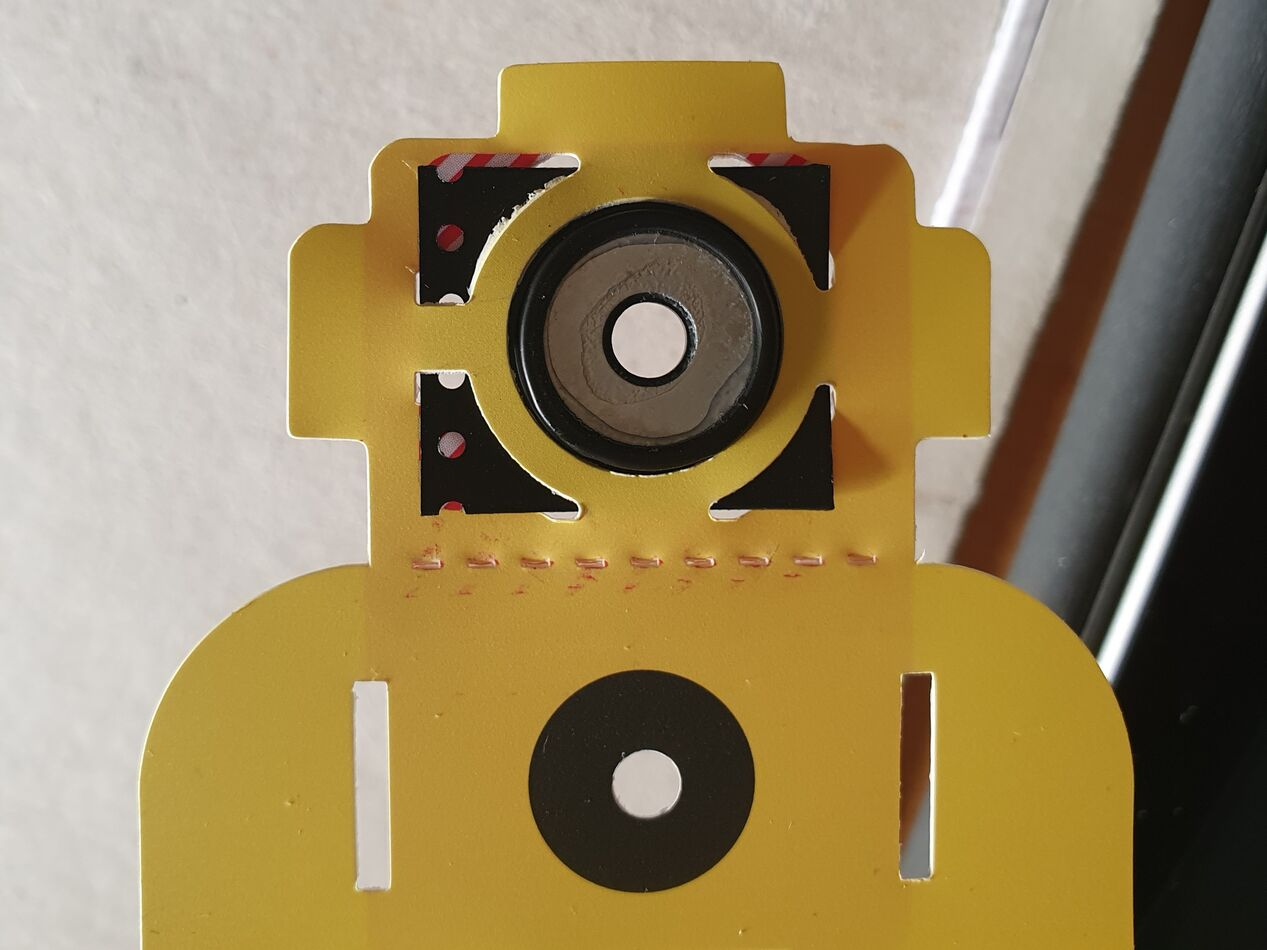
\includegraphics[width=0.3\textwidth]{images/aufbau/2_3.jpg} &
				\multicolumn{1}{l|}{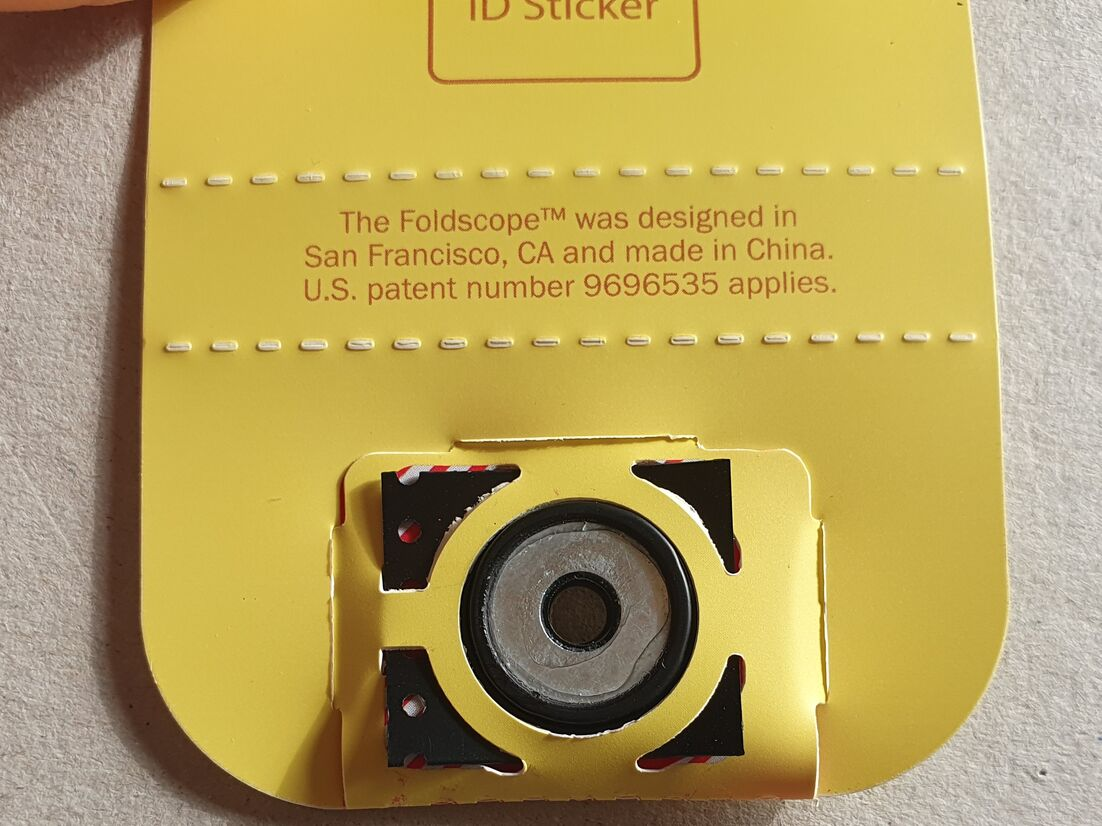
\includegraphics[width=0.3\textwidth]{images/aufbau/2_4.jpg}} &
				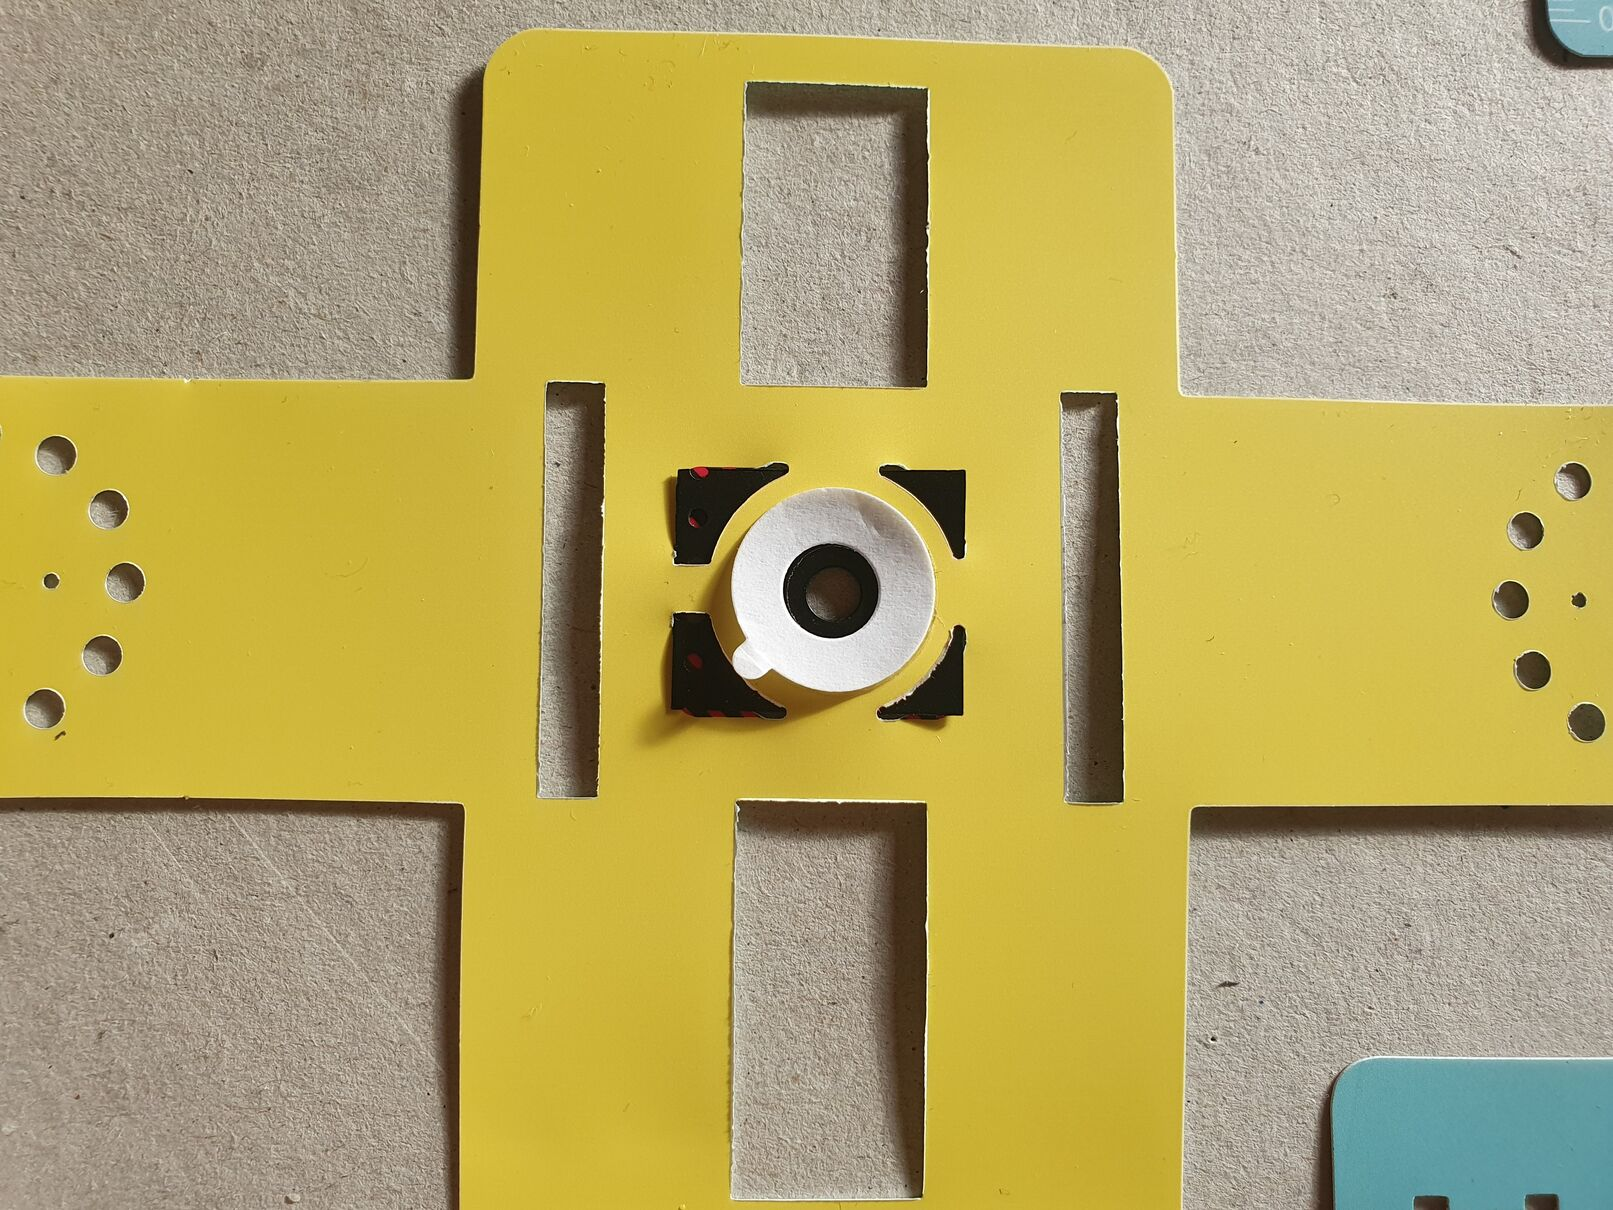
\includegraphics[width=0.3\textwidth]{images/aufbau/3_1.jpg} 
				\\
				% \bottomrule
				\\[-0.5em]
				% \toprule
				$\rightarrow$ & \multicolumn{1}{l|}{$\rightarrow$} & Schritt 4 \\
				\midrule
				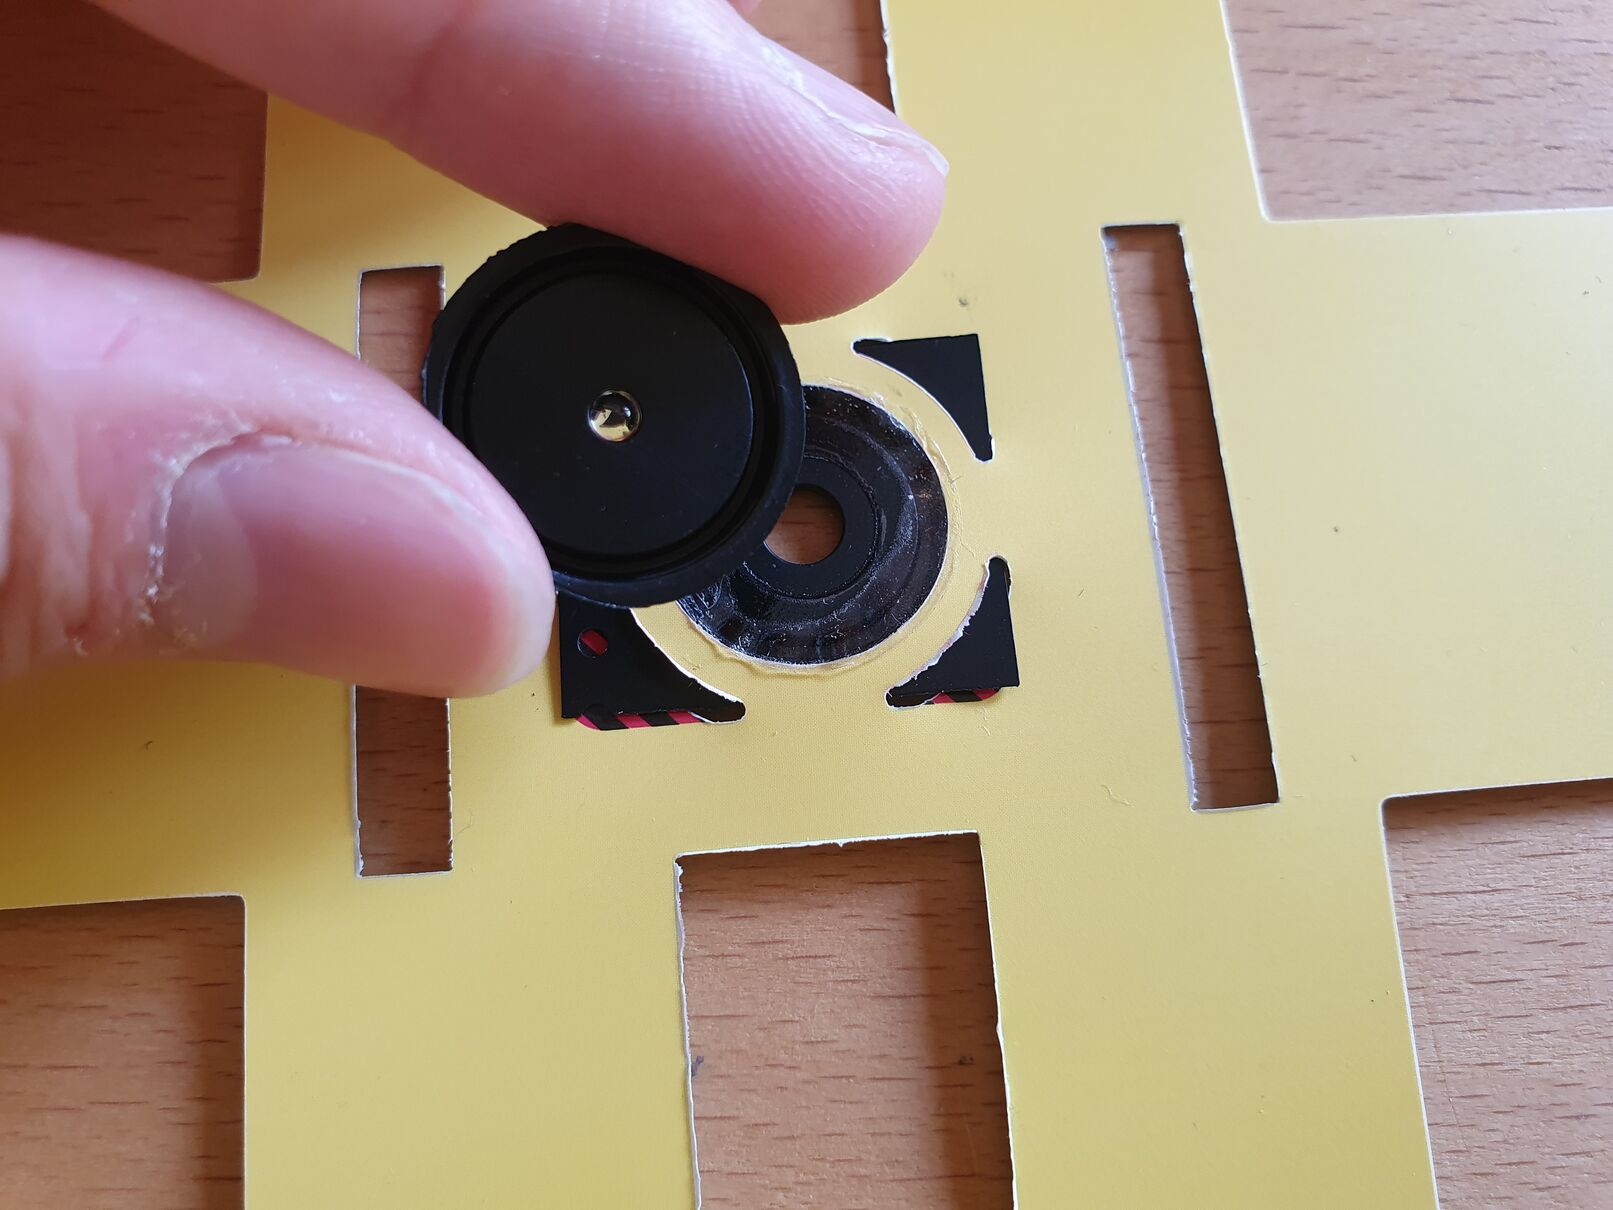
\includegraphics[width=0.3\textwidth]{images/aufbau/3_2.jpg} &
				\multicolumn{1}{l|}{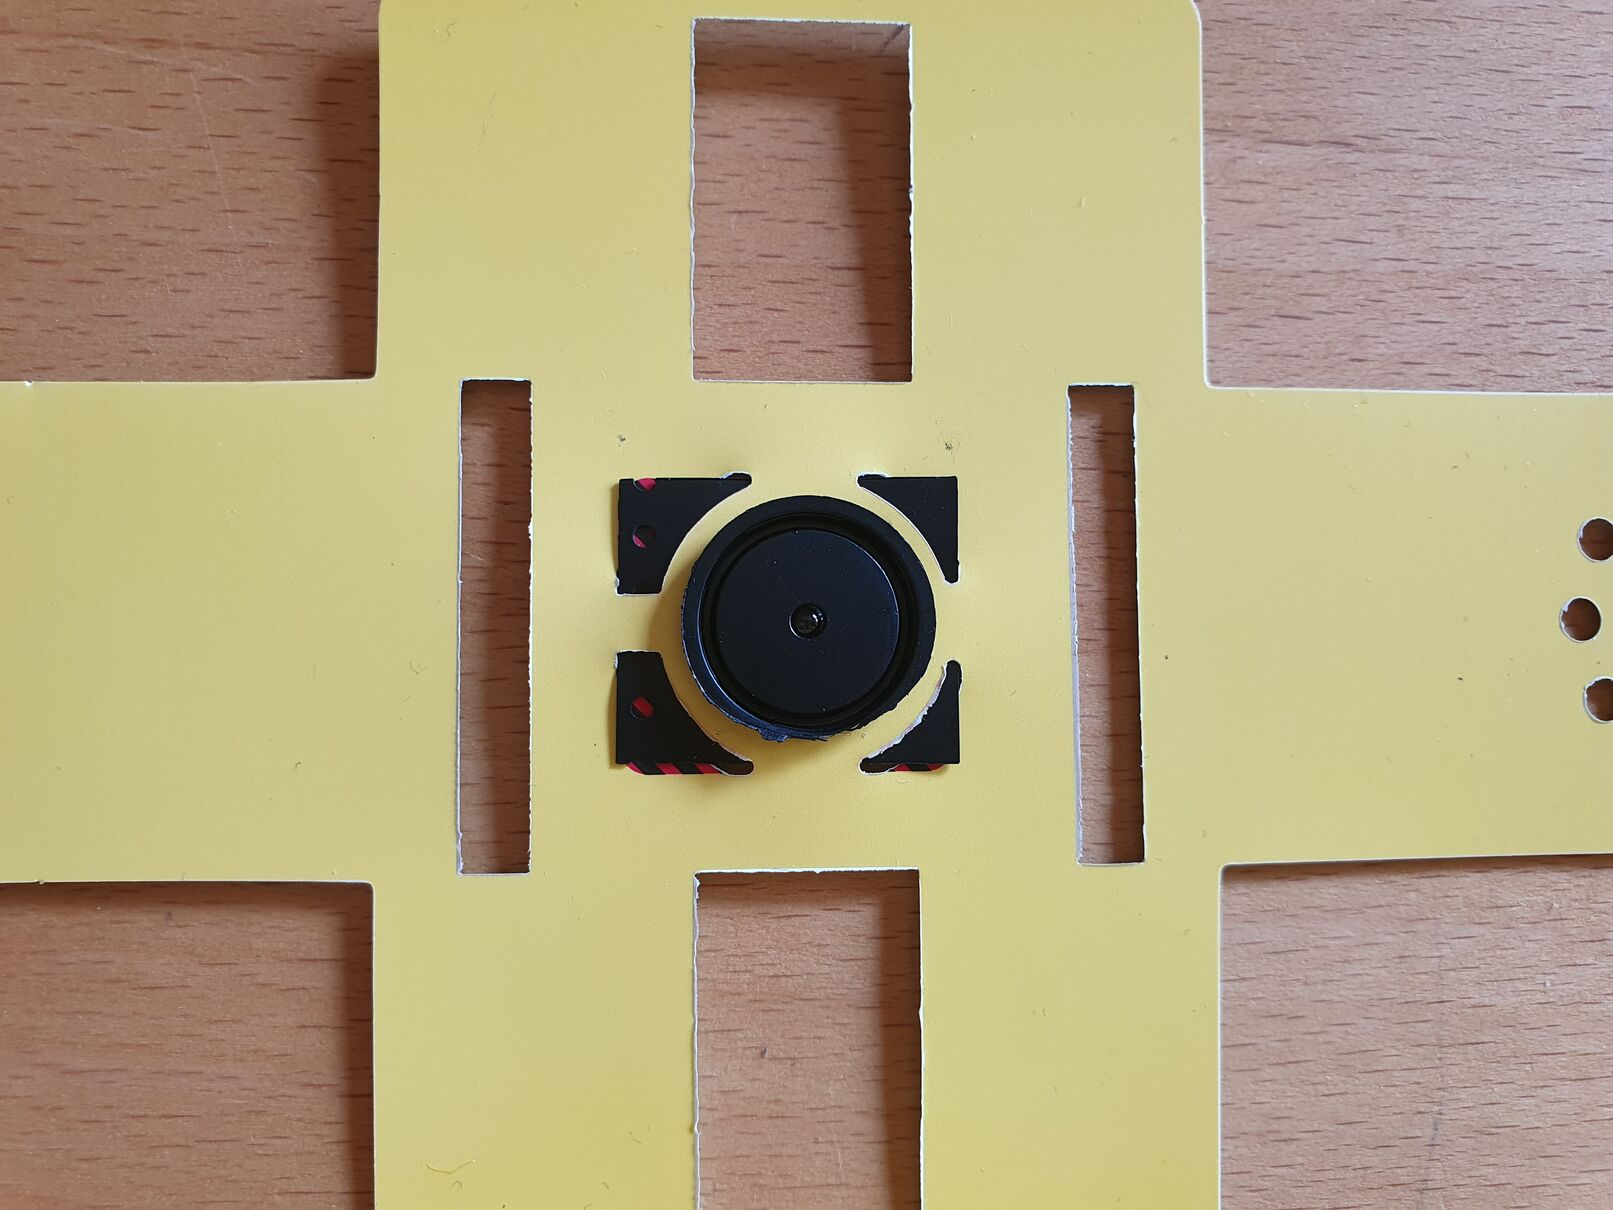
\includegraphics[width=0.3\textwidth]{images/aufbau/3_3.jpg}} &
				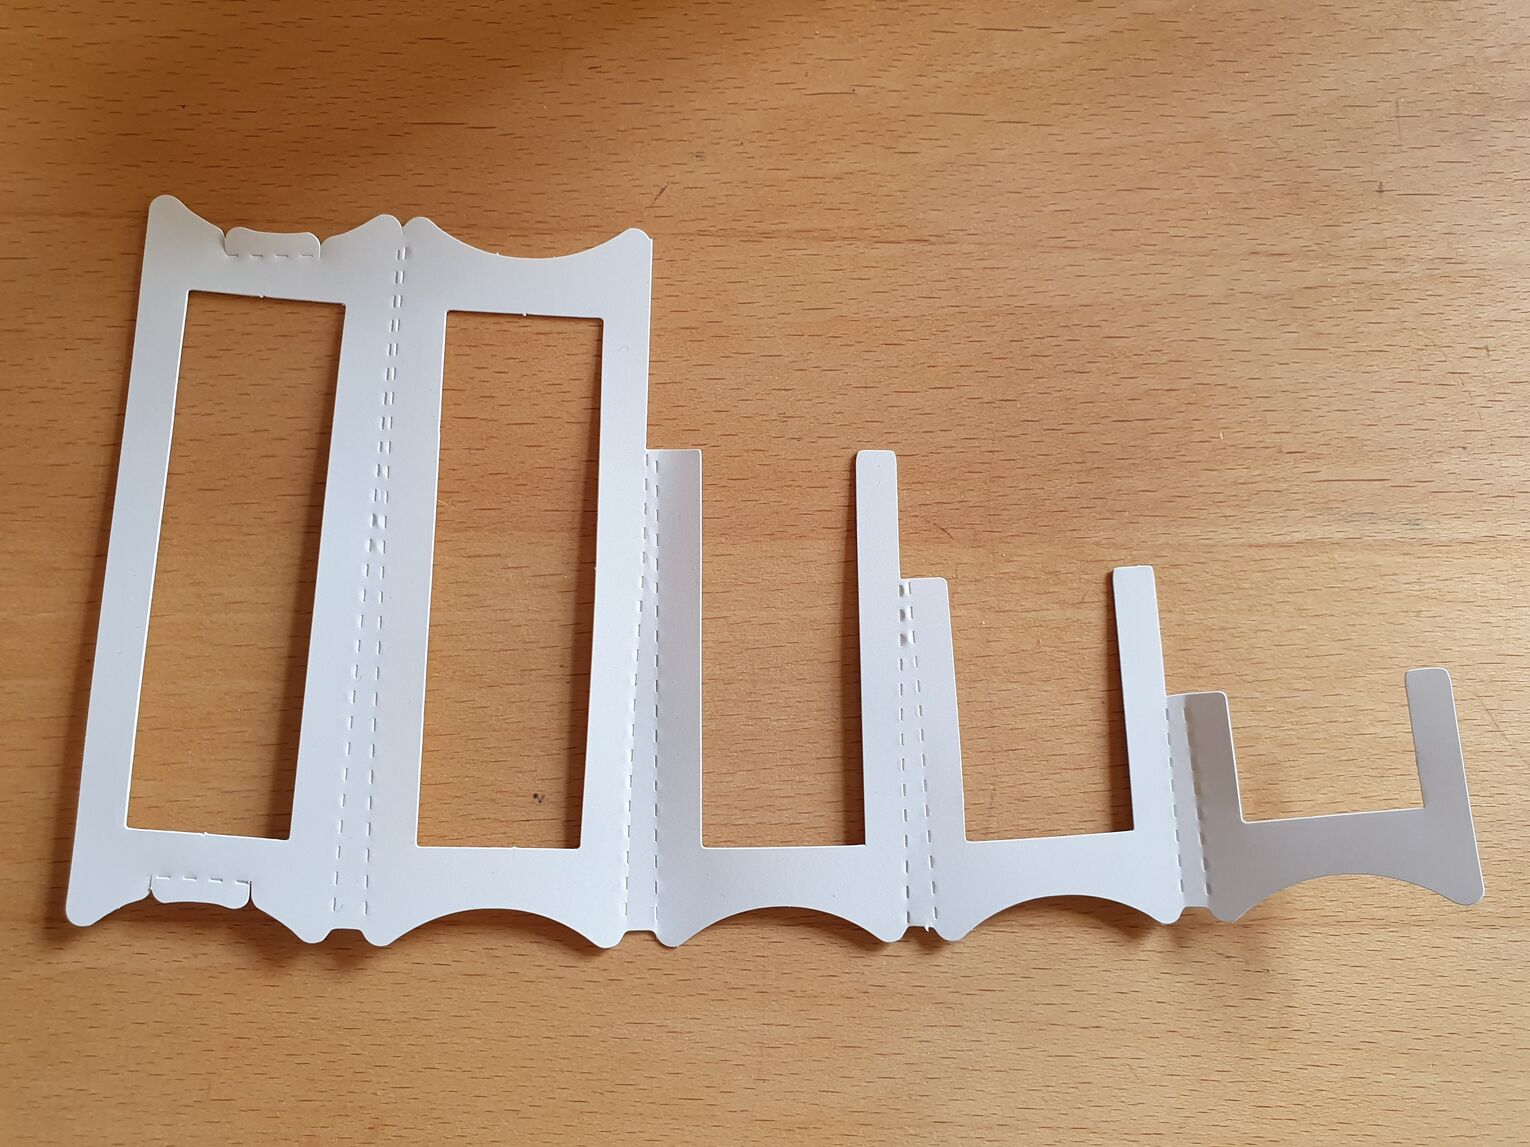
\includegraphics[width=0.3\textwidth]{images/aufbau/4_1.jpg} 
				\\
				% \bottomrule
			\end{tabular}
		\end{center}
		\vfill
		\newpage
		\begin{center}
			\begin{tabular}{l|l|l}
				% \toprule
				\multicolumn{1}{l}{$\rightarrow$} & $\rightarrow$ & Schritt 5 \\
				\midrule
				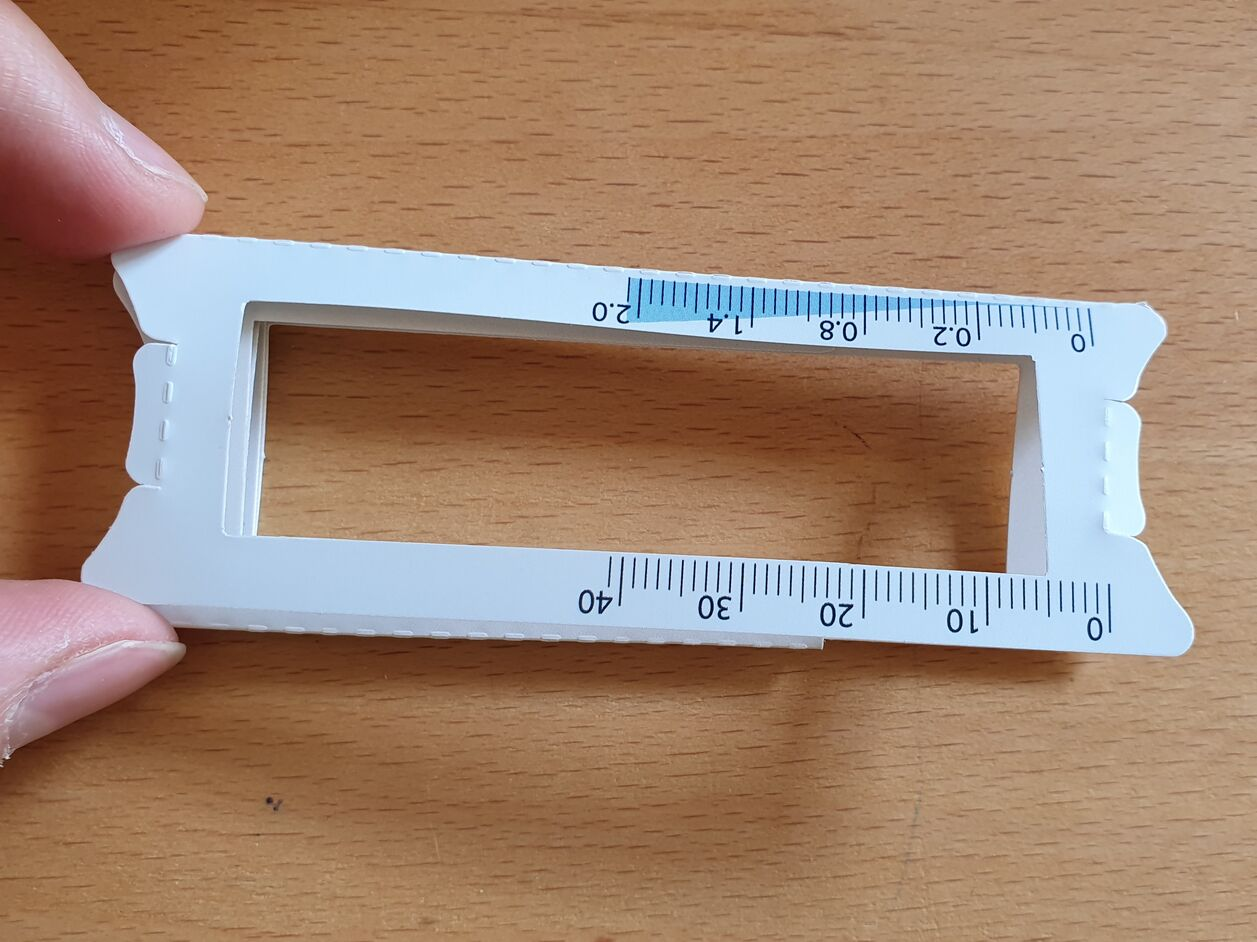
\includegraphics[width=0.3\textwidth]{images/aufbau/4_2.jpg} &
				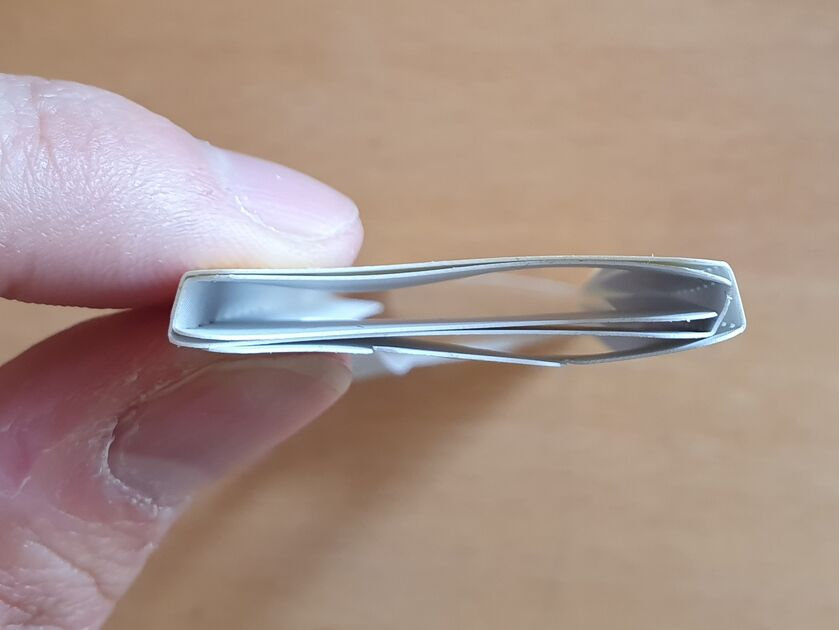
\includegraphics[width=0.3\textwidth]{images/aufbau/4_3.jpg} &
				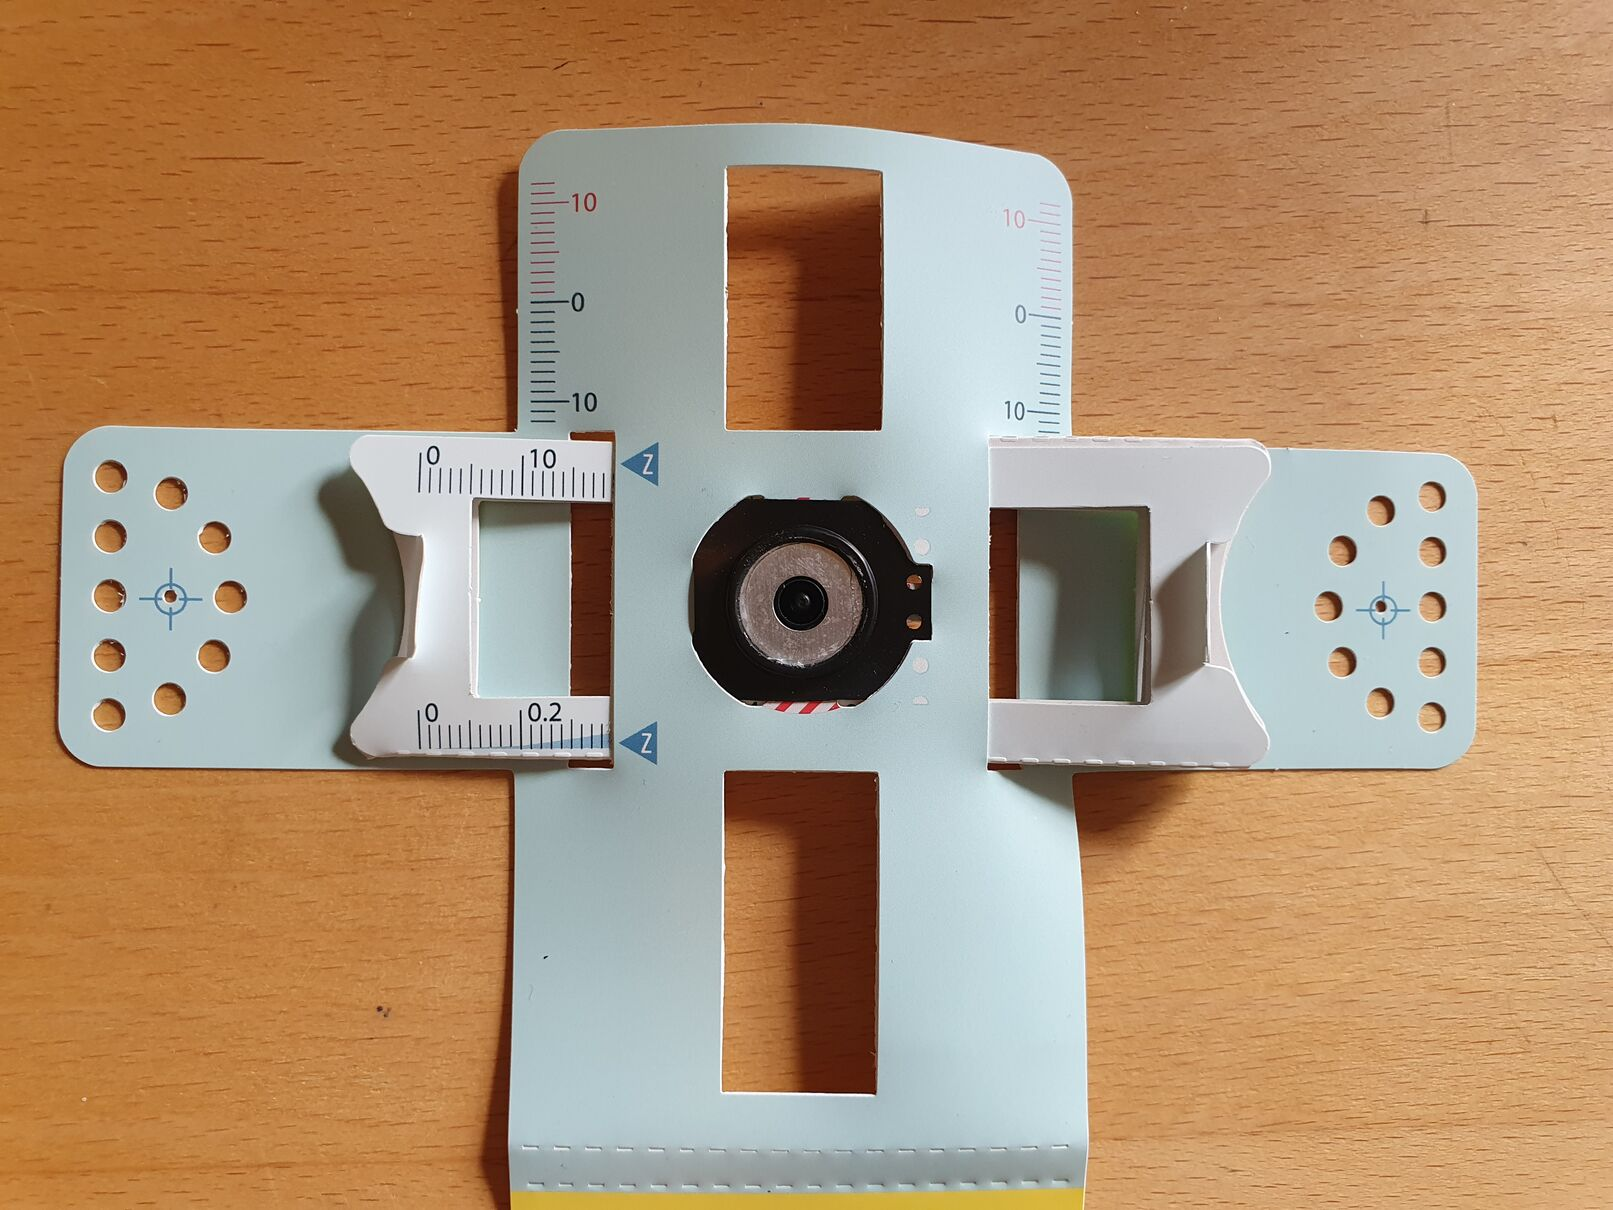
\includegraphics[width=0.3\textwidth]{images/aufbau/5.jpg} \\
				% \bottomrule
				\multicolumn{3}{l}{} \\[-0.5em]
				% \toprule
				Schritt 6 & Schritt 7 & Schritt 8  \\
				\midrule
				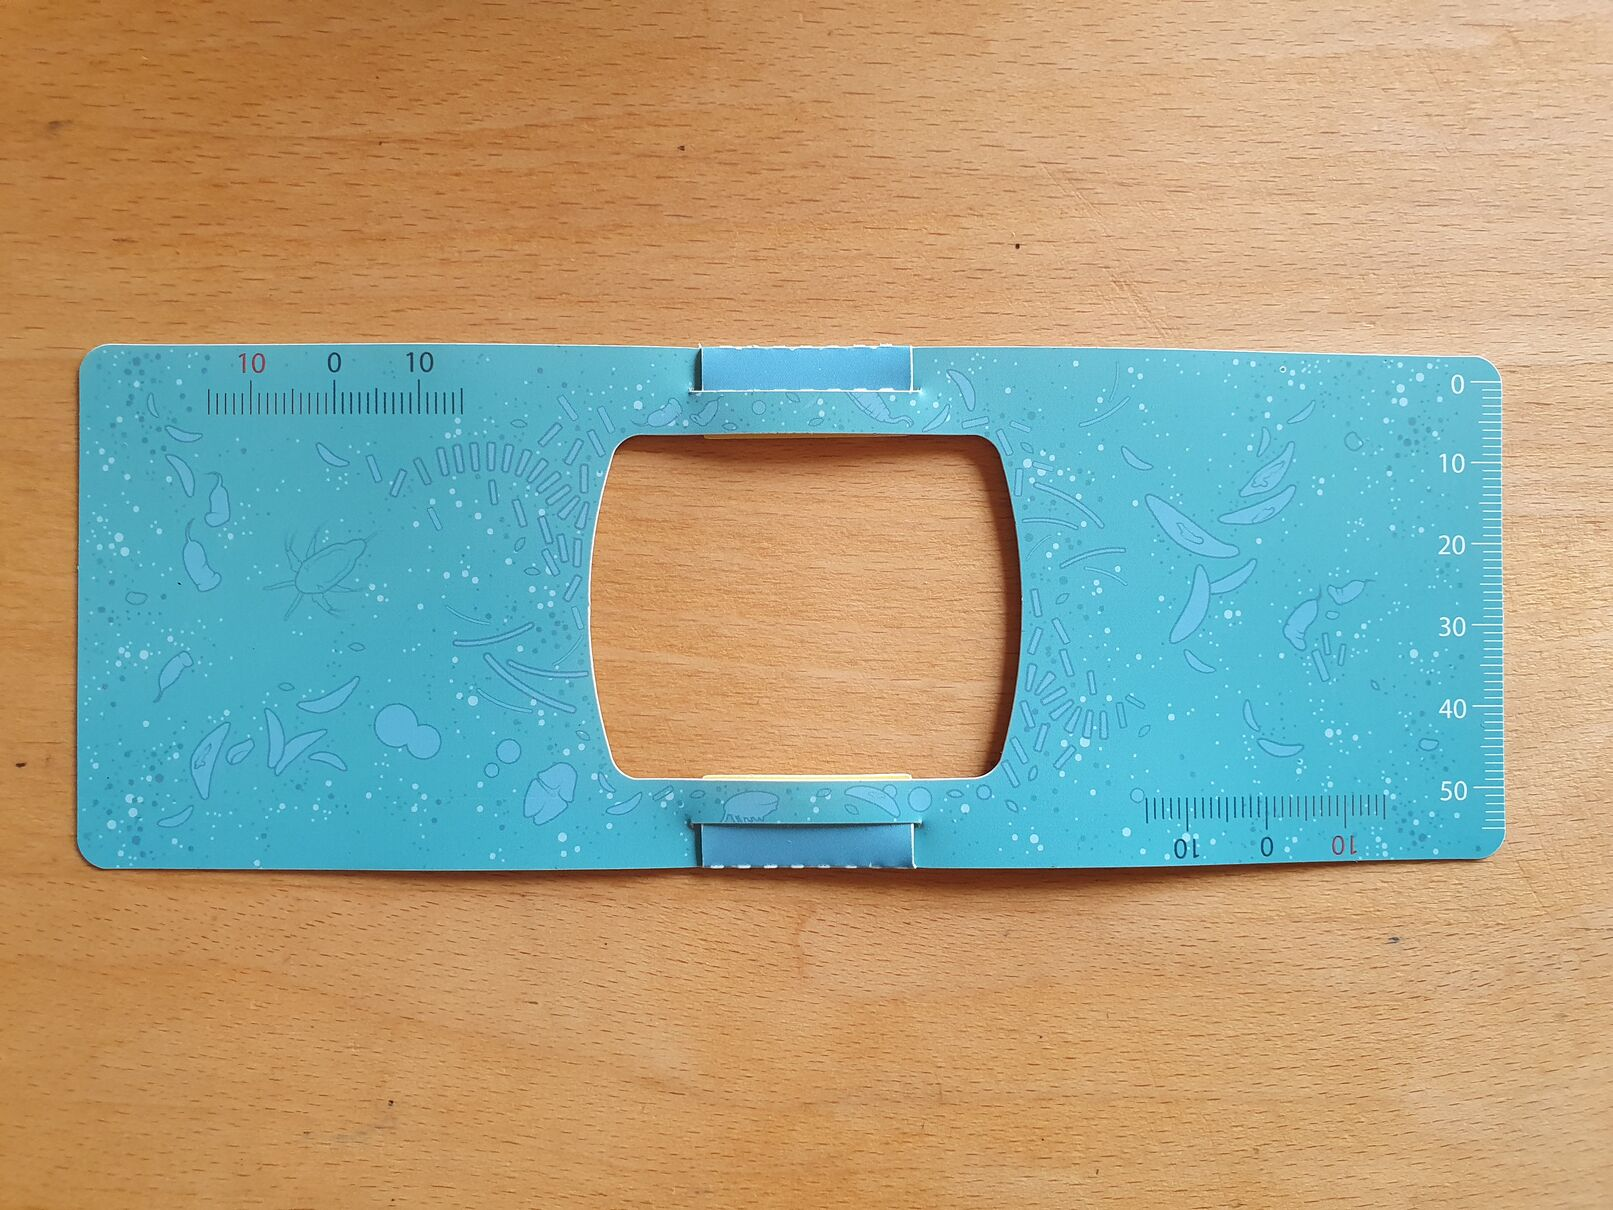
\includegraphics[width=0.3\textwidth]{images/aufbau/6.jpg} &
				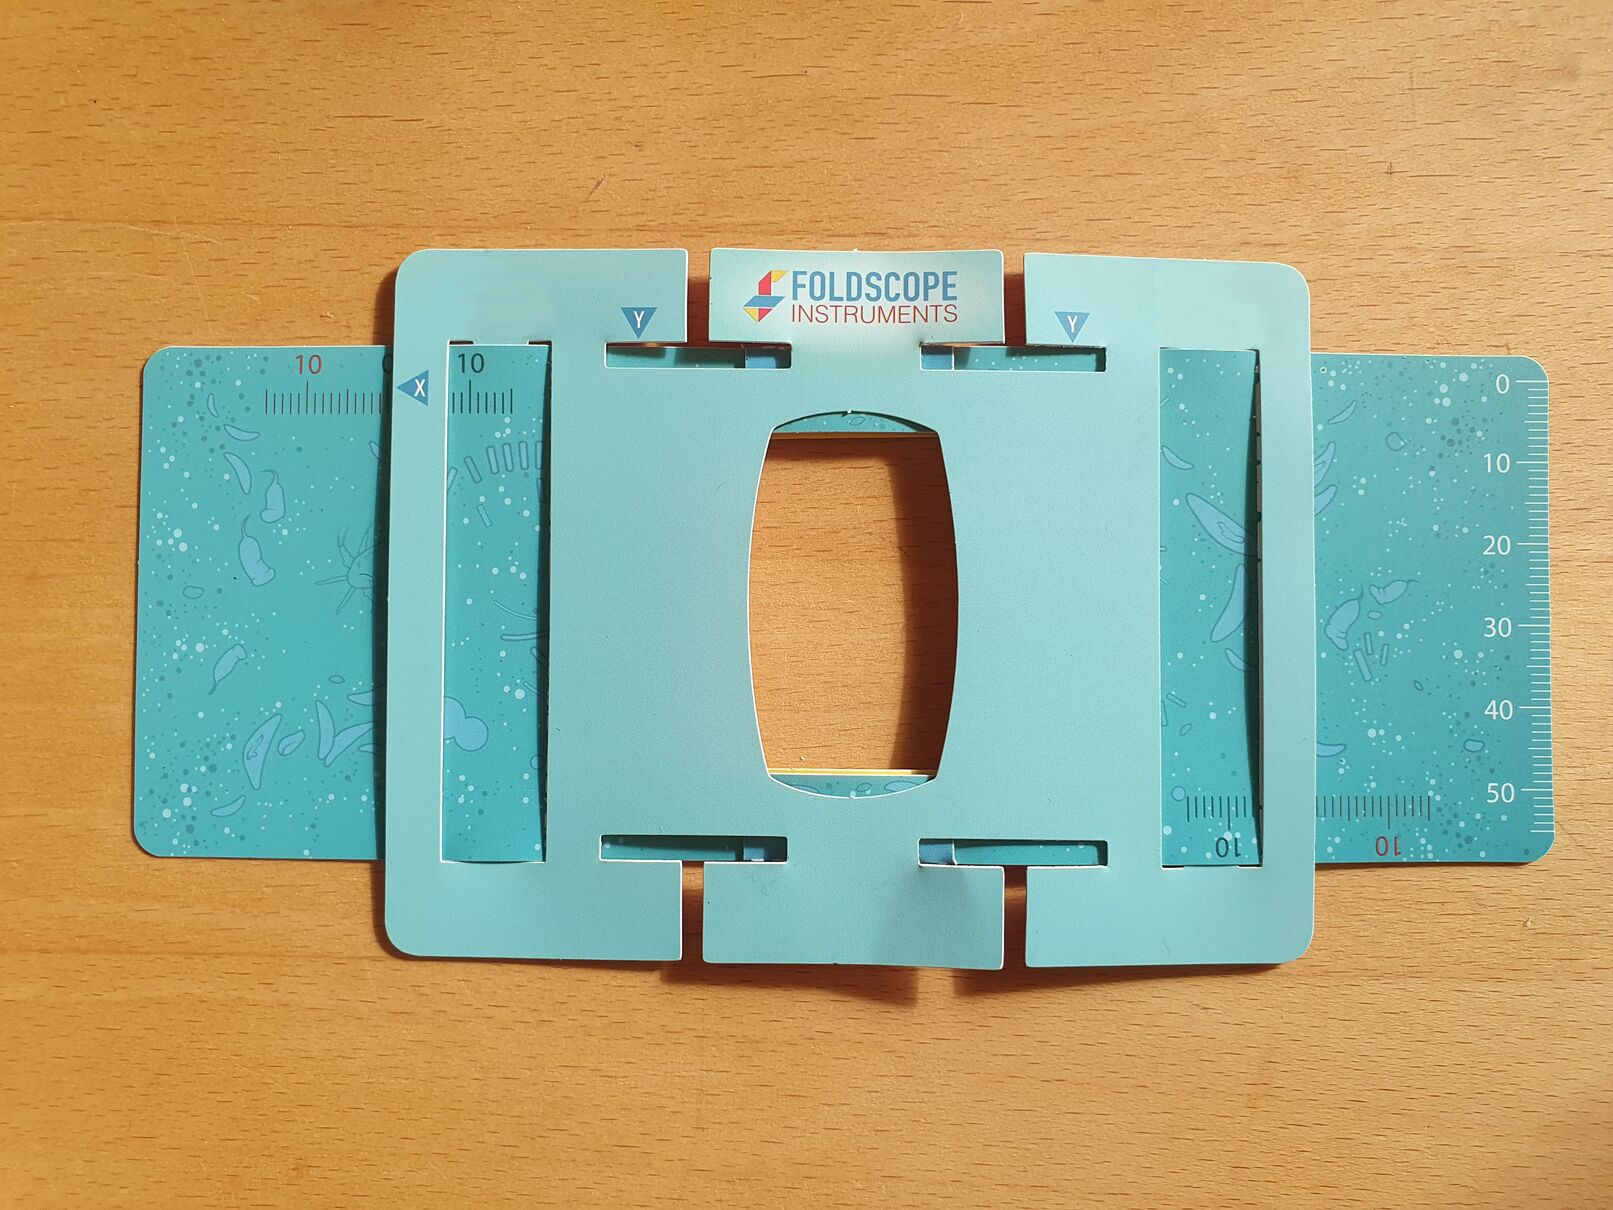
\includegraphics[width=0.3\textwidth]{images/aufbau/7.jpg} &
				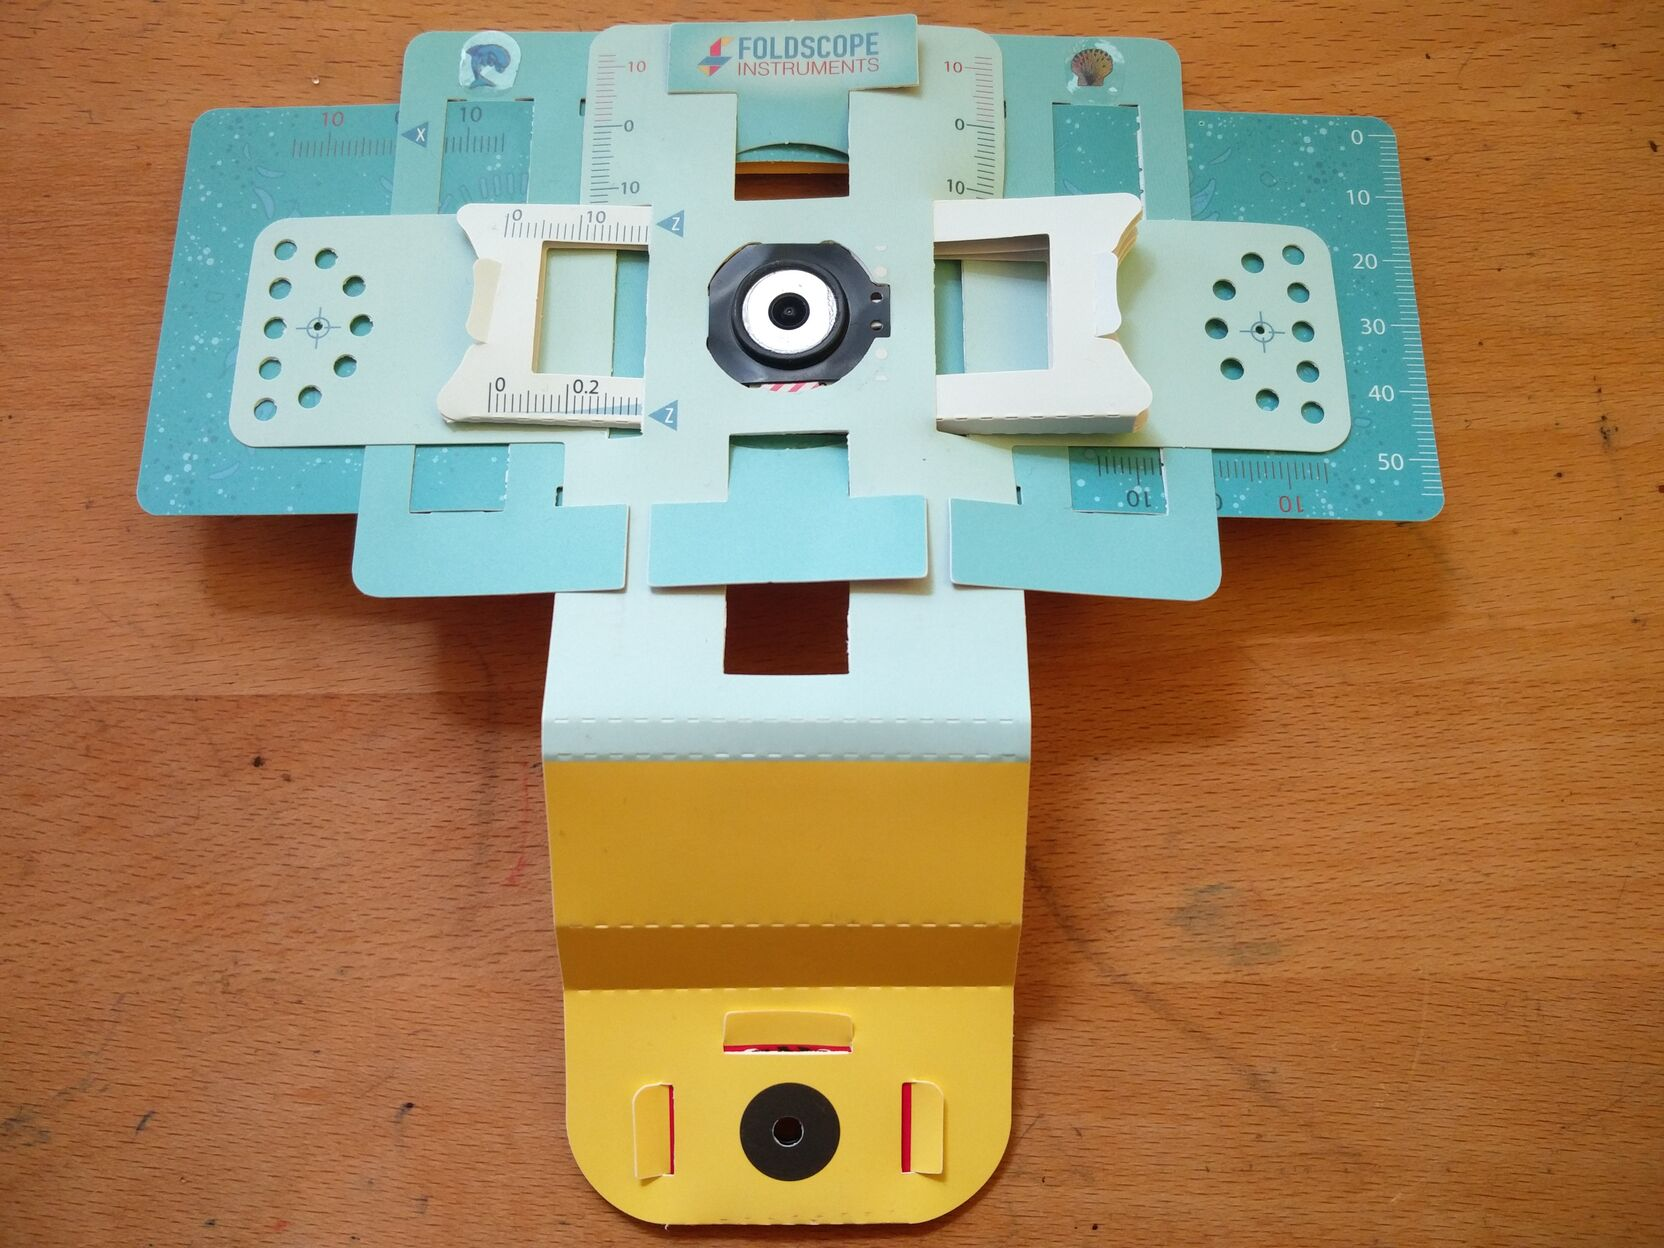
\includegraphics[width=0.3\textwidth]{images/aufbau/8.jpg} \\
				% \bottomrule
				\multicolumn{3}{l}{} \\[-0.5em]
				% \toprule
				Schritt 9 & Schritt 10 & Fertig \\
				\midrule
				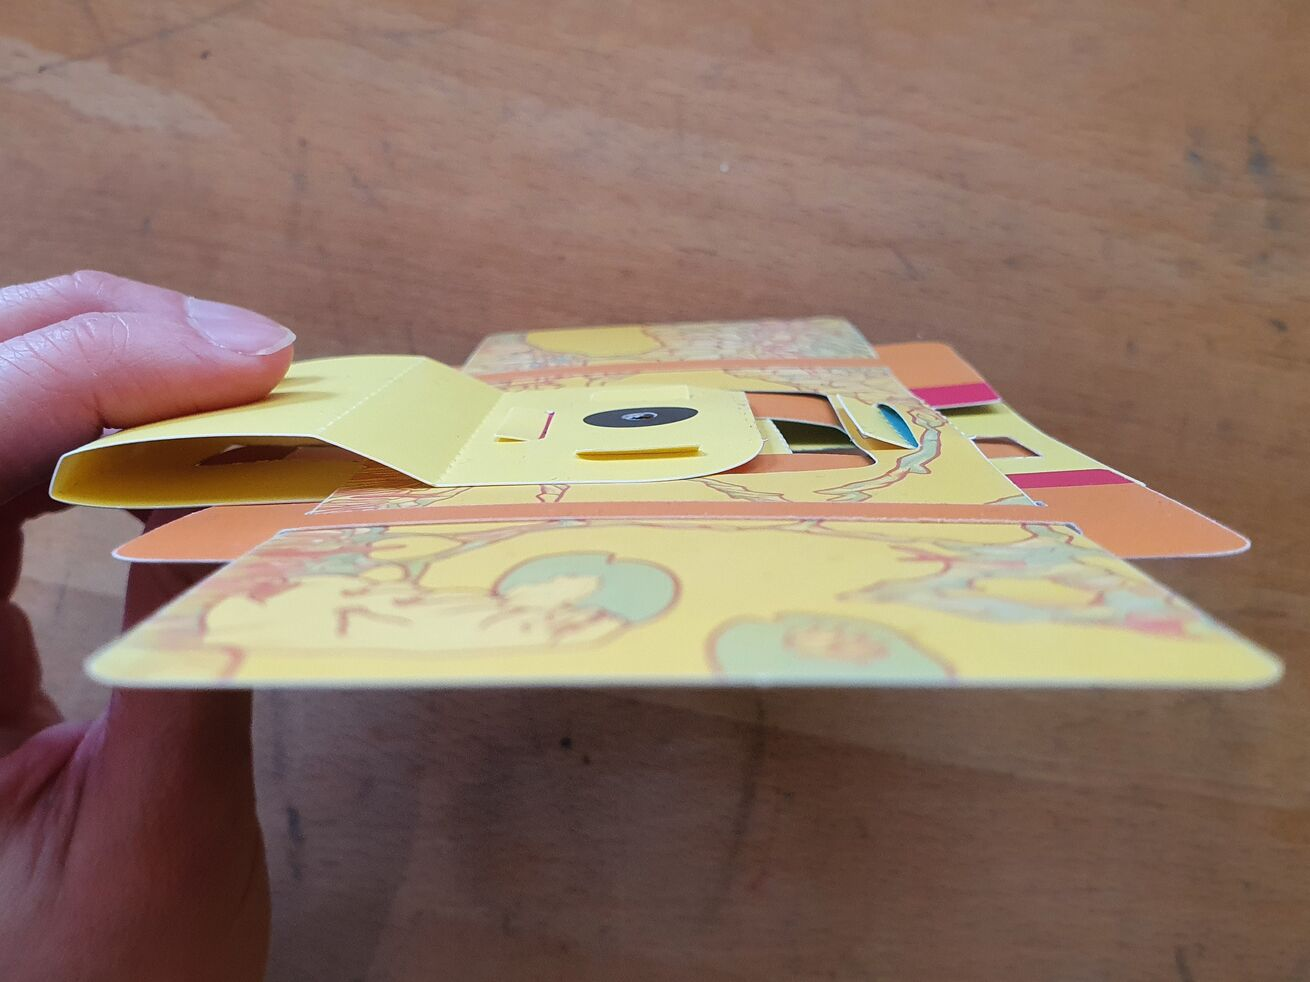
\includegraphics[width=0.3\textwidth]{images/aufbau/9.jpg} &
				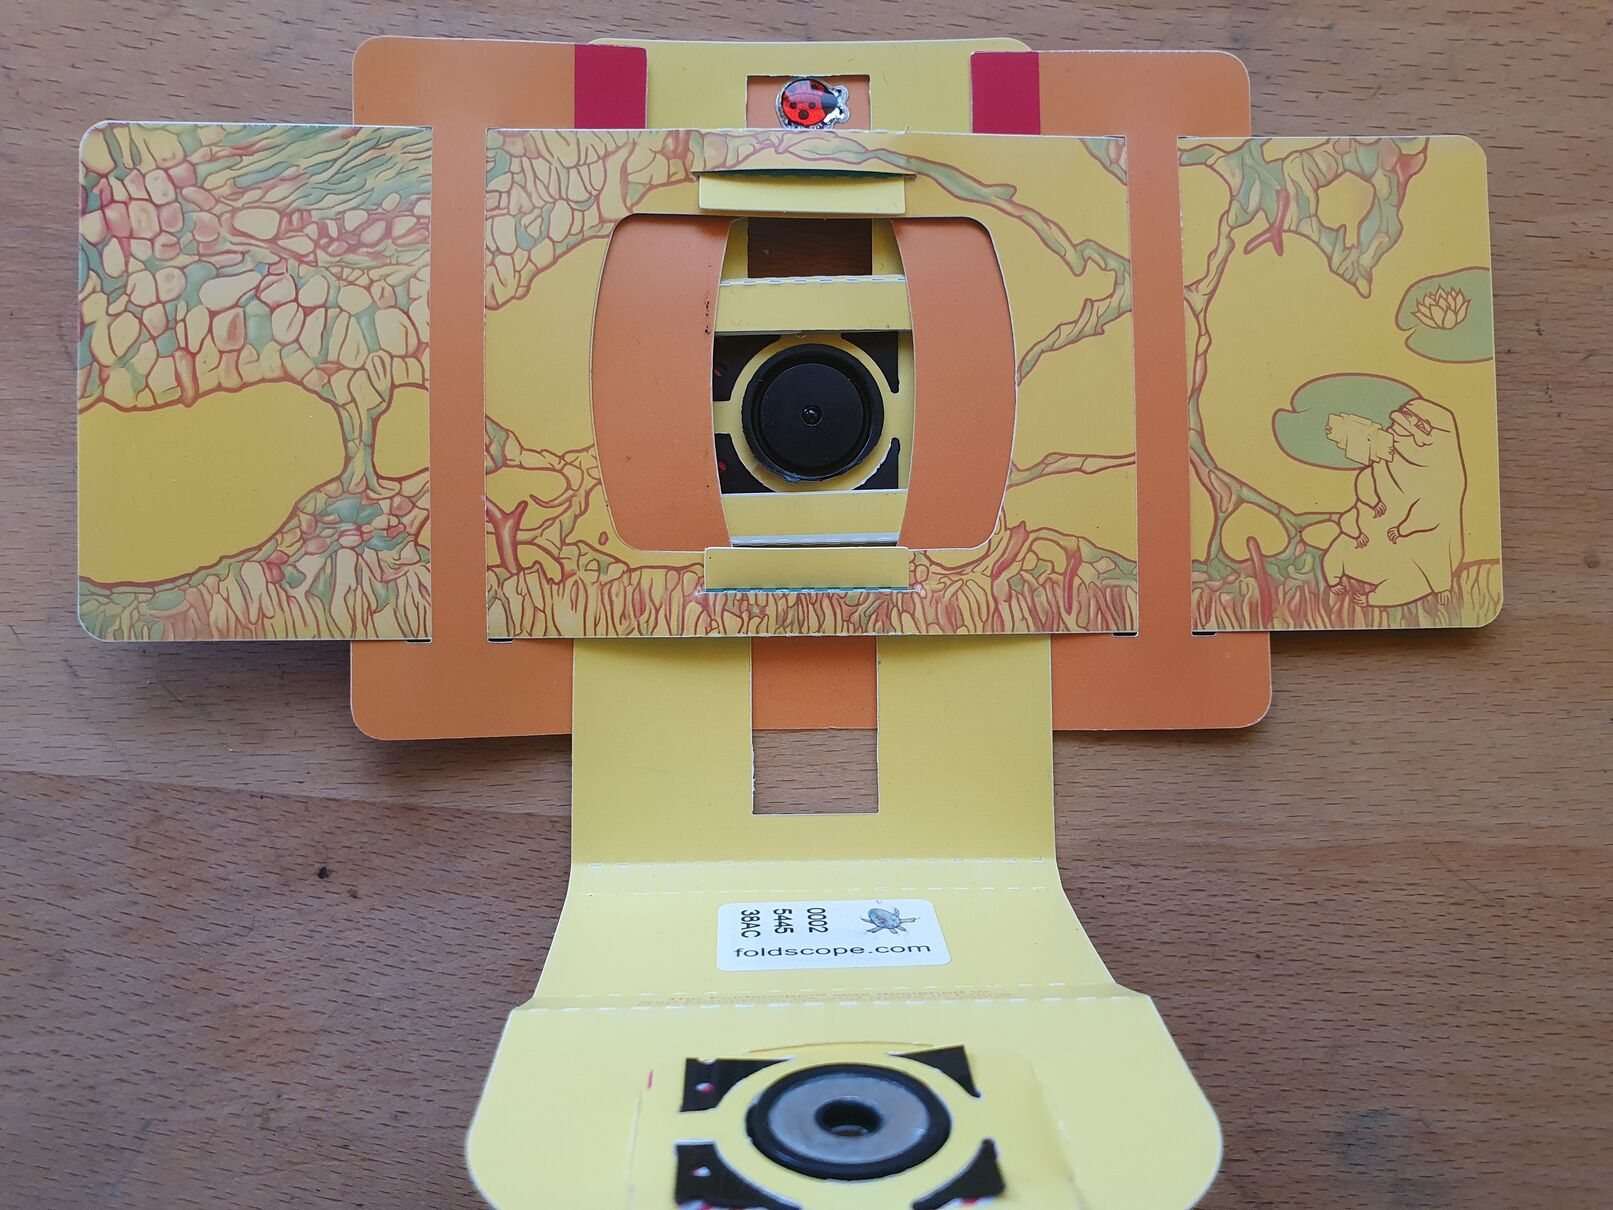
\includegraphics[width=0.3\textwidth]{images/aufbau/10.jpg} & 
				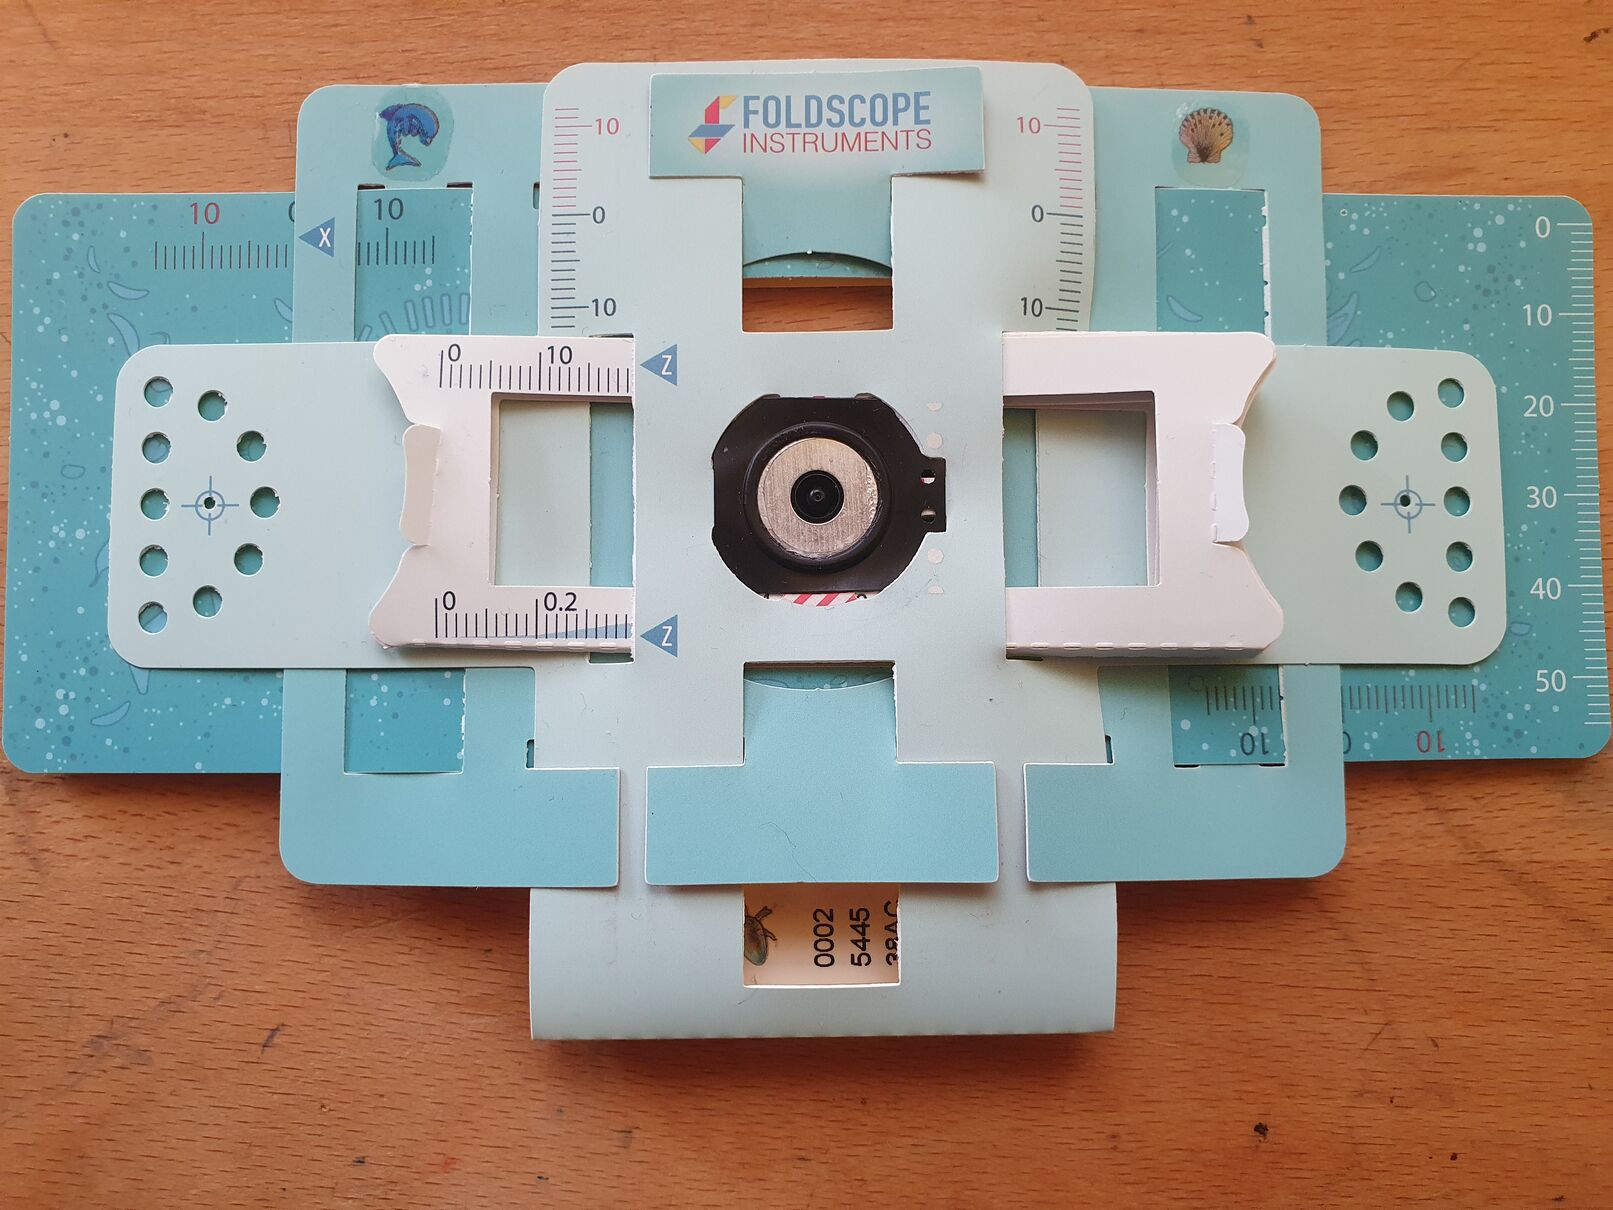
\includegraphics[width=0.3\textwidth]{images/aufbau/fertig.jpg} \\
				% \bottomrule
			\end{tabular}
		\end{center}
		\vspace{1em}
		Im Schritt 10 ("Foldscope individualisieren") haben wir zusätzlich mit Aufkleber unsere Foldscopes verziert. Mein fertiges Foldscope sieht dann so aus:
		\begin{figure}[H]
			\centering
			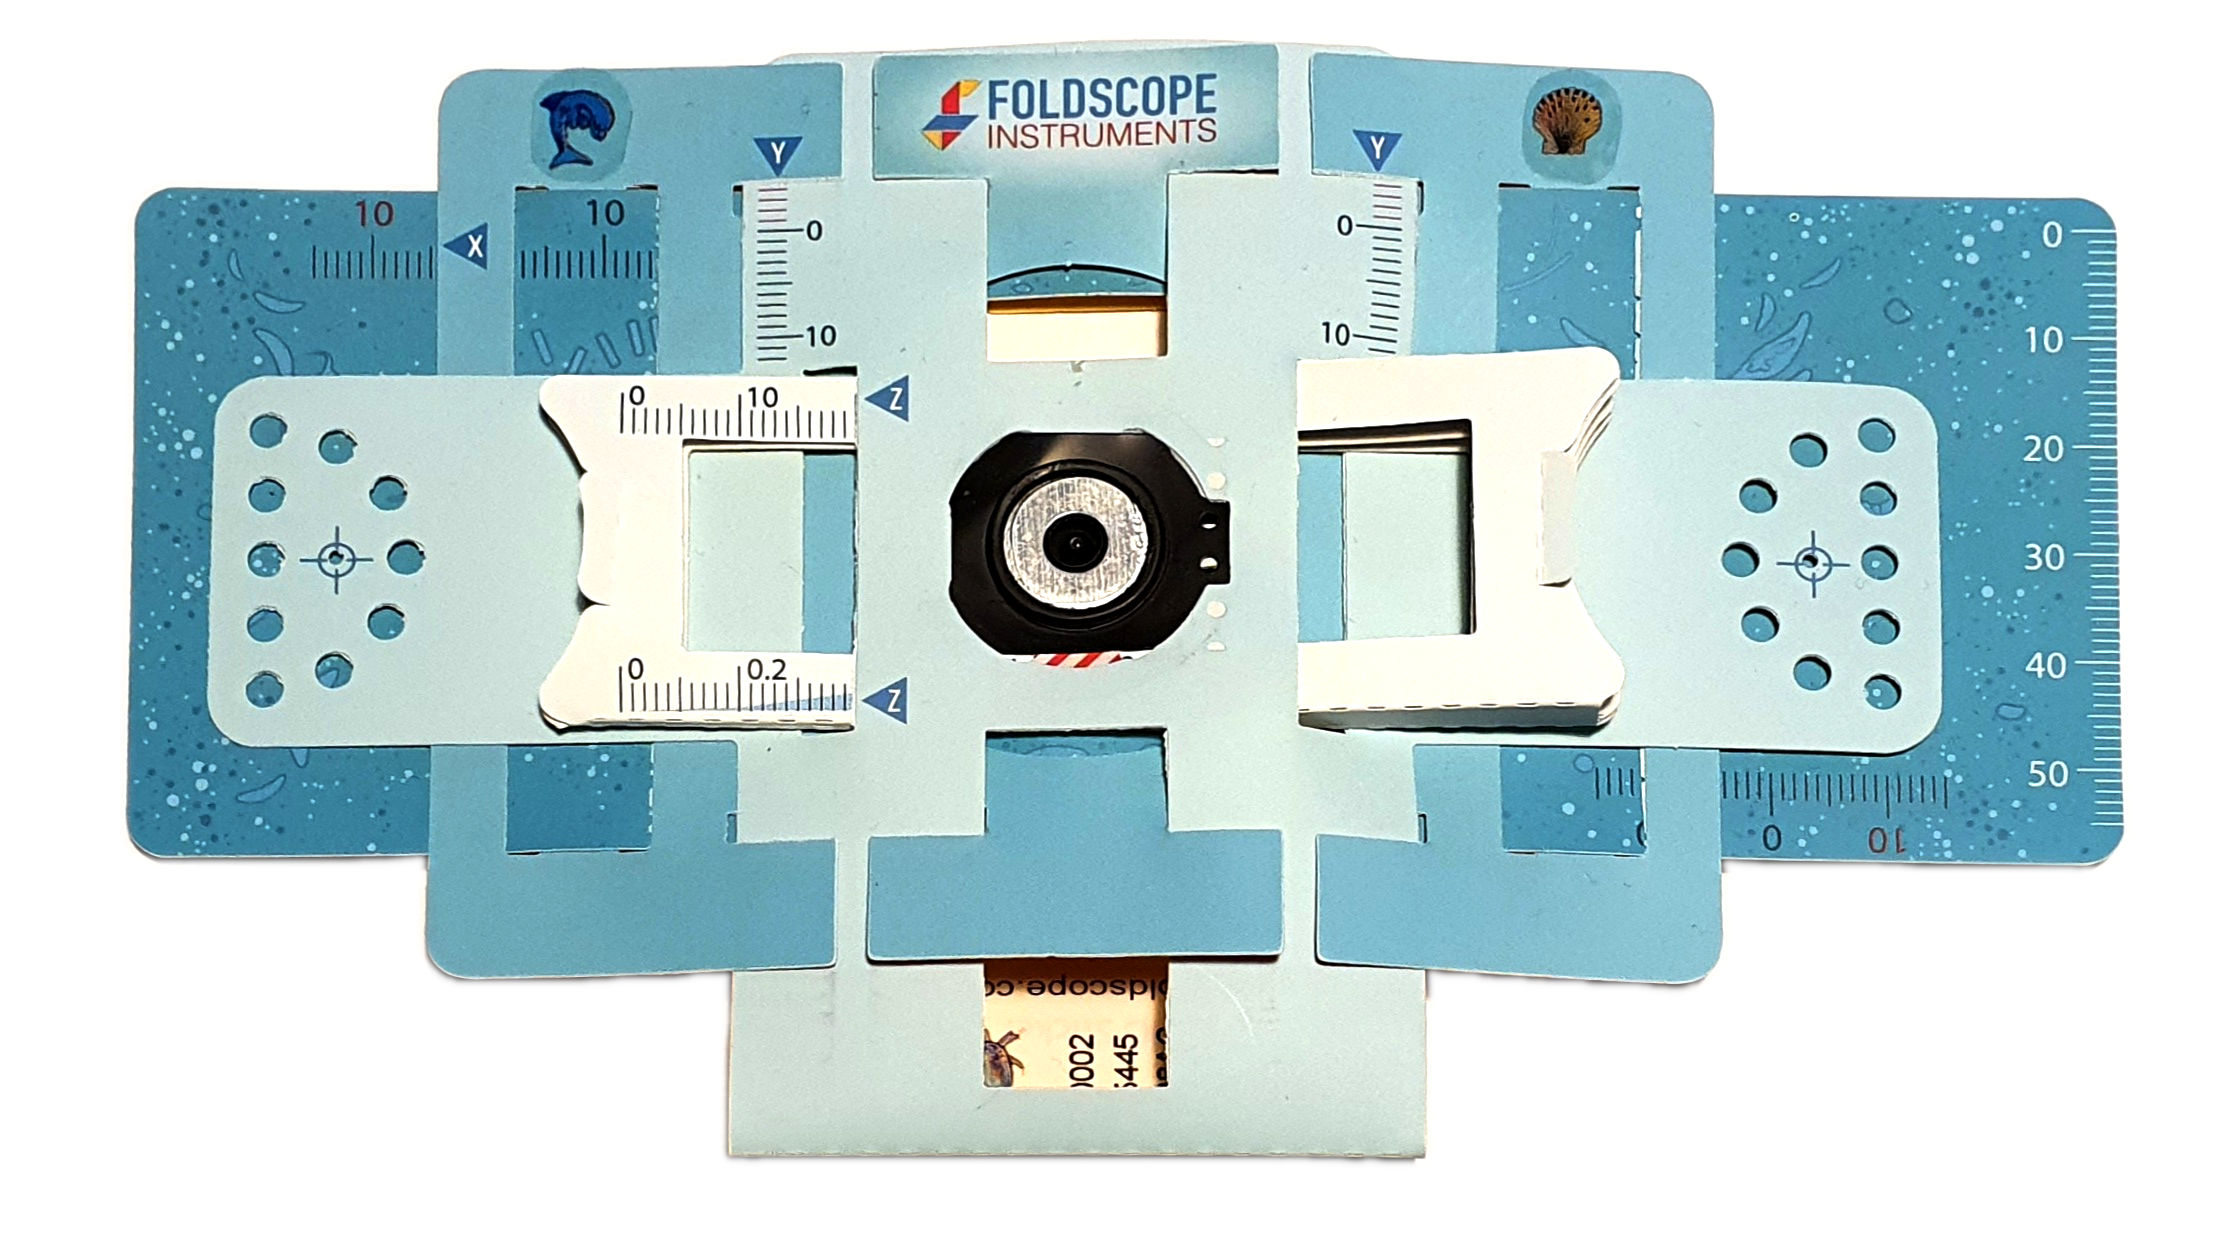
\includegraphics[width=0.6\textwidth]{cover.jpg}
			\caption{\centering Foldscope \texttt{0002} \texttt{5445} \texttt{38AC}}
		\end{figure}
